\documentclass[11pt,a4paper]{article}

\usepackage[utf8]{inputenc}
\usepackage[T1]{fontenc}
\usepackage[french]{babel}
\usepackage[margin=2.5cm]{geometry}

\usepackage{amsmath}
\usepackage{amssymb}
\usepackage{booktabs}
\usepackage{graphicx}
\usepackage{hyperref}
\usepackage{siunitx}

\sisetup{
  output-decimal-marker = {,},
  per-mode = symbol
}

\title{Cadre méthodologique SCCI-2026 : dérivation variationnelle, couplage TOV--champ et contribution dipolaire}
\author{Mohamed Nour Kayad (SCCI-2026)}
\date{\today}

\begin{document}

\maketitle

\begin{abstract}
Nous présentons le cadre méthodologique du modèle SCCI-2026 pour l'étude de la contribution dipolaire $\dot P_b^{\mathrm{dip}}$ dans les systèmes binaires à pulsar. Le texte articule l'action effective, l'équation d'Euler--Lagrange du champ $\Phi$, le statut de la paramétrisation polynomiale $\mathfrak R(\Phi)=1+\eta\Phi^2$ sous l'hypothèse d'identification $\mathfrak R\equiv Z_A$, la définition opérationnelle des sensibilités effectives $\alpha_i$ et de l'écart $\Delta\alpha=\alpha_B-\alpha_A$, la résolution couplée des équations d'hydrostatique relativiste de type Tolman--Oppenheimer--Volkoff modifiées, les garde-fous perturbatifs, le statut du repère méthodologique interne de \SI{1e-13}{\second\per\second} et les conditions d'une confrontation observationnelle par chronométrie des pulsars.
\end{abstract}

\section{Pipeline numérique de sensibilité et reproductibilité}

Les balayages combinés de sensibilité ont été réalisés avec \texttt{pulsar\_field\_sweep.py} et \texttt{pulsar\_field\_sweep\_polynomial.py}. Les cartes associées ont été générées par \texttt{plot\_pulsar\_field\_heatmap.py} et \texttt{plot\_pulsar\_field\_heatmap\_polynomial.py}.

Les tableaux de résultats sont fournis dans \texttt{results/} et archivés dans \texttt{data/processed/}, avec un manifeste d'intégrité \texttt{metadata.json} contenant les empreintes SHA-256 des fichiers CSV.

Ces sorties constituent des analyses de sensibilité paramétrique évaluées par rapport au repère interne de \SI{1e-13}{\second\per\second}, et non des contraintes observationnelles.

\begin{figure}[htbp]
  \centering
  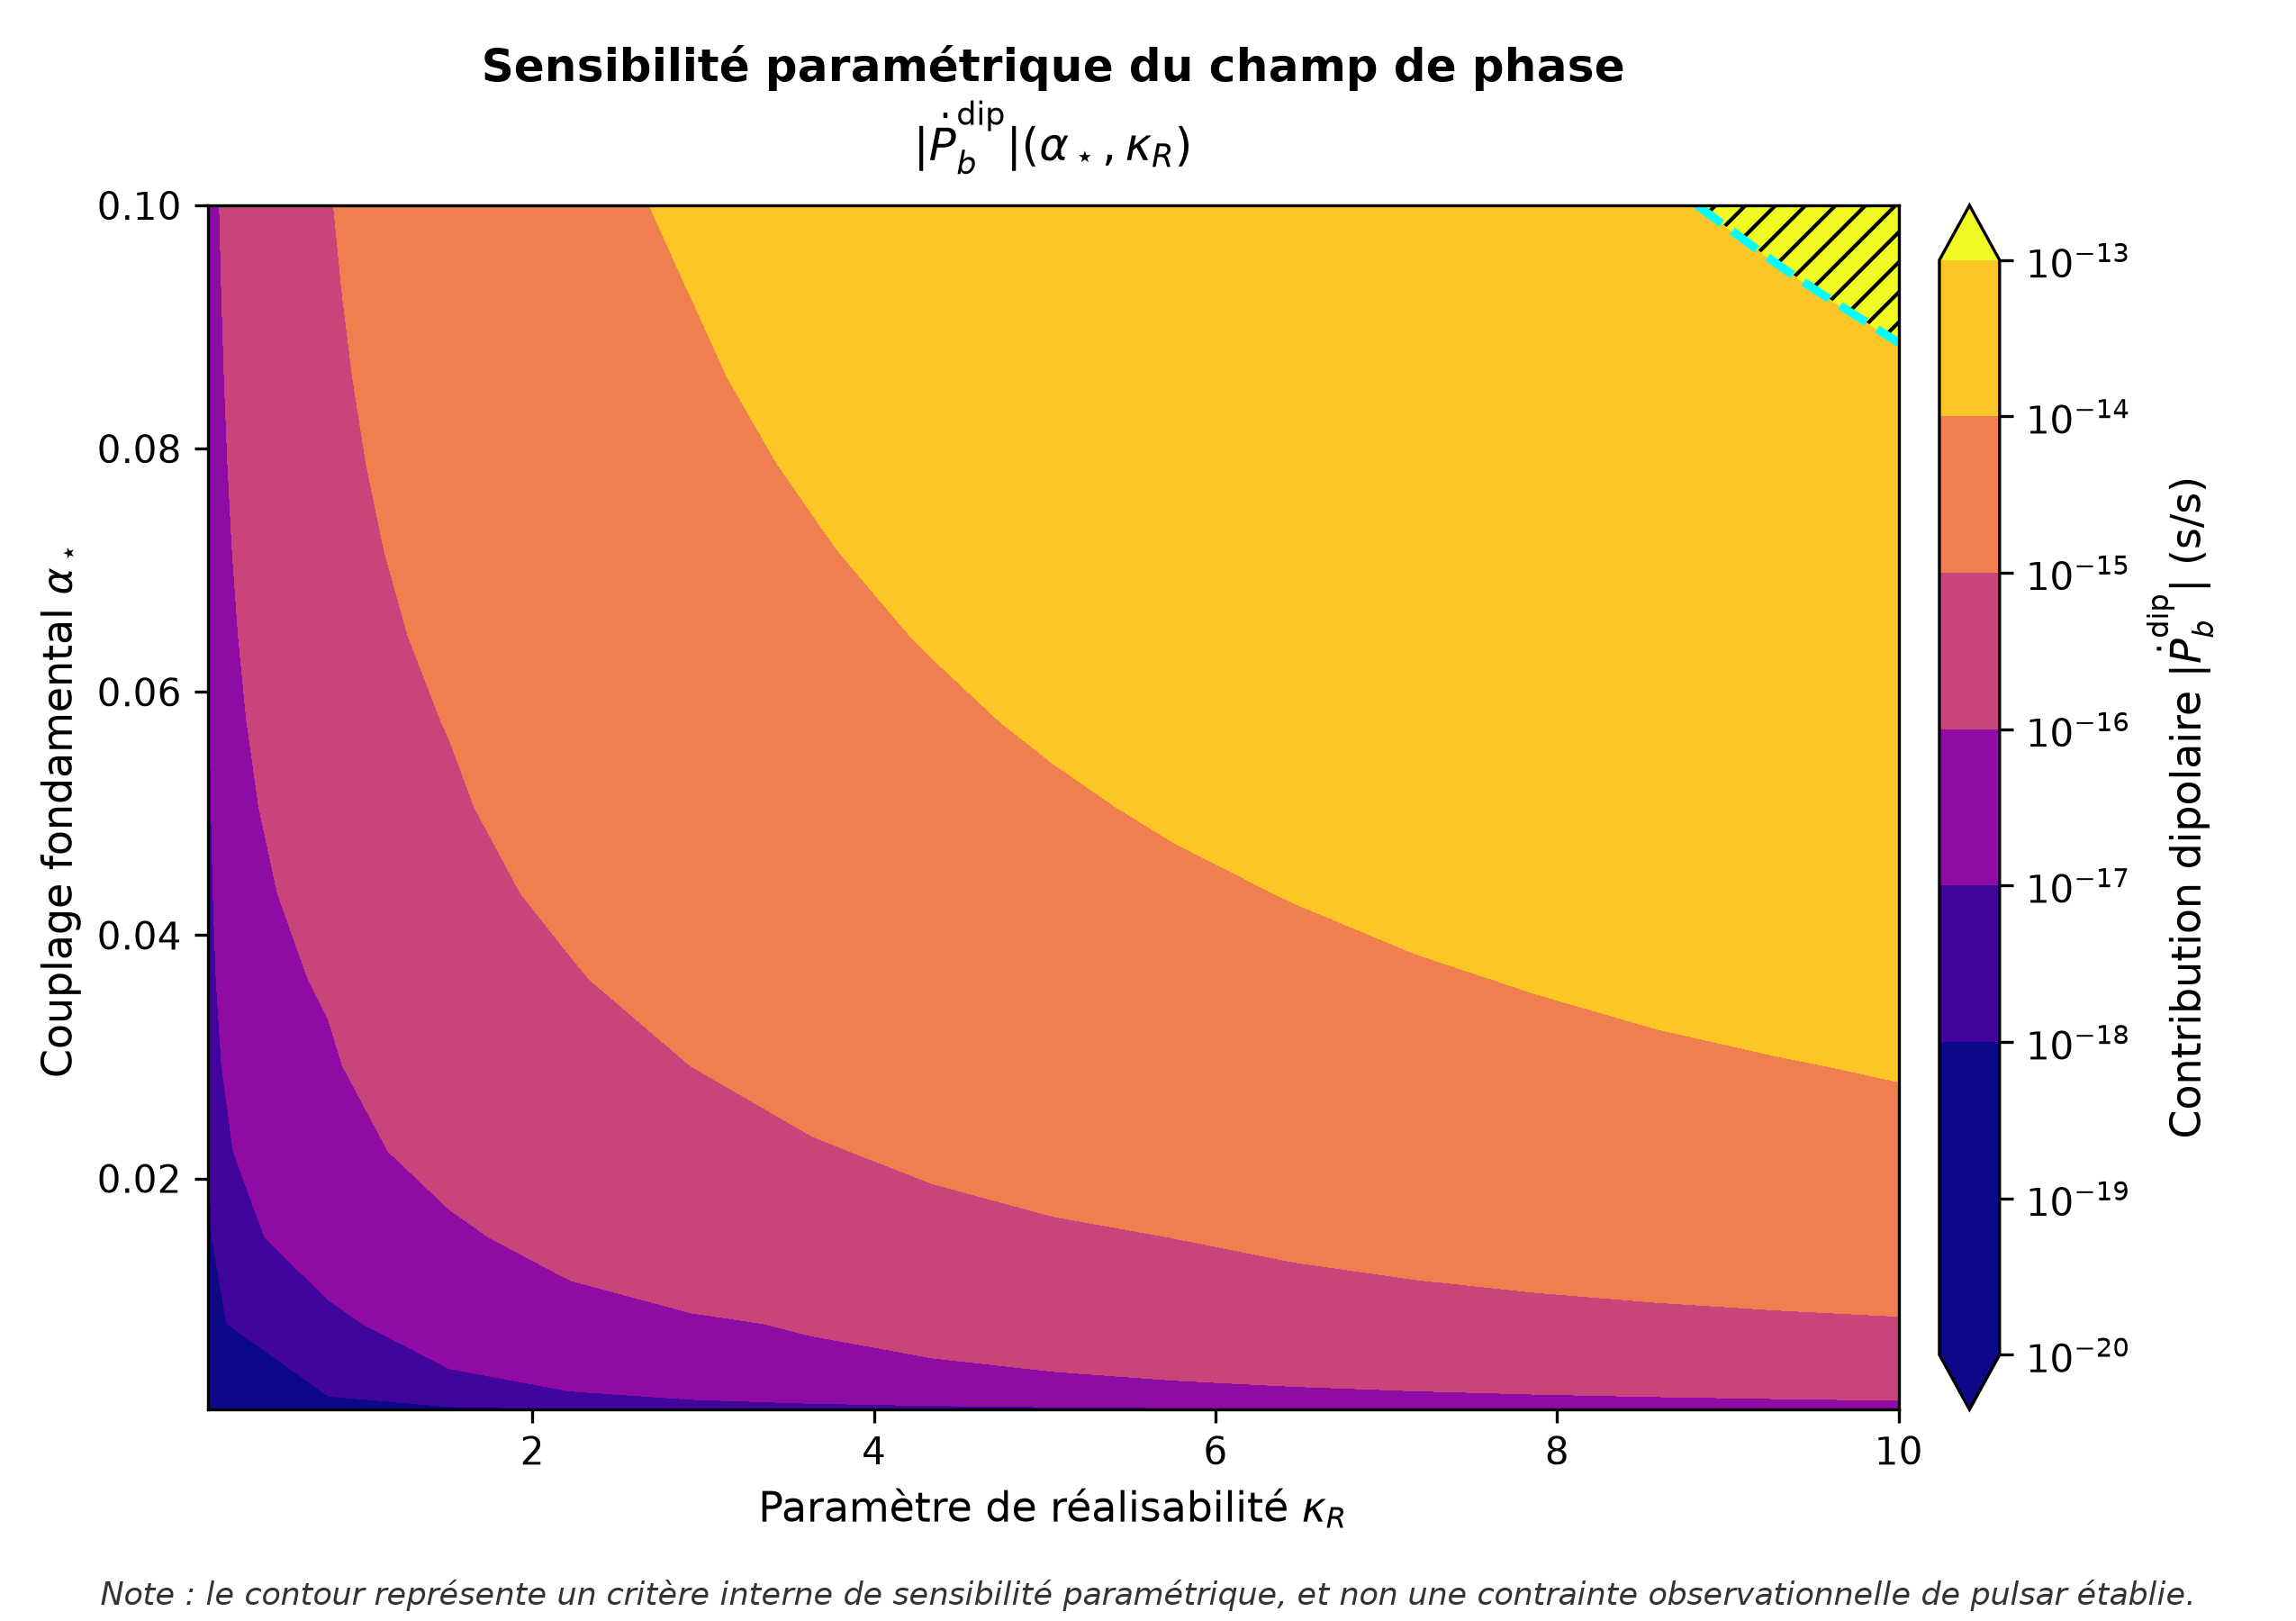
\includegraphics[width=0.48\textwidth]{figures/pulsar_field_sensitivity_heatmap.png}
  \hfill
  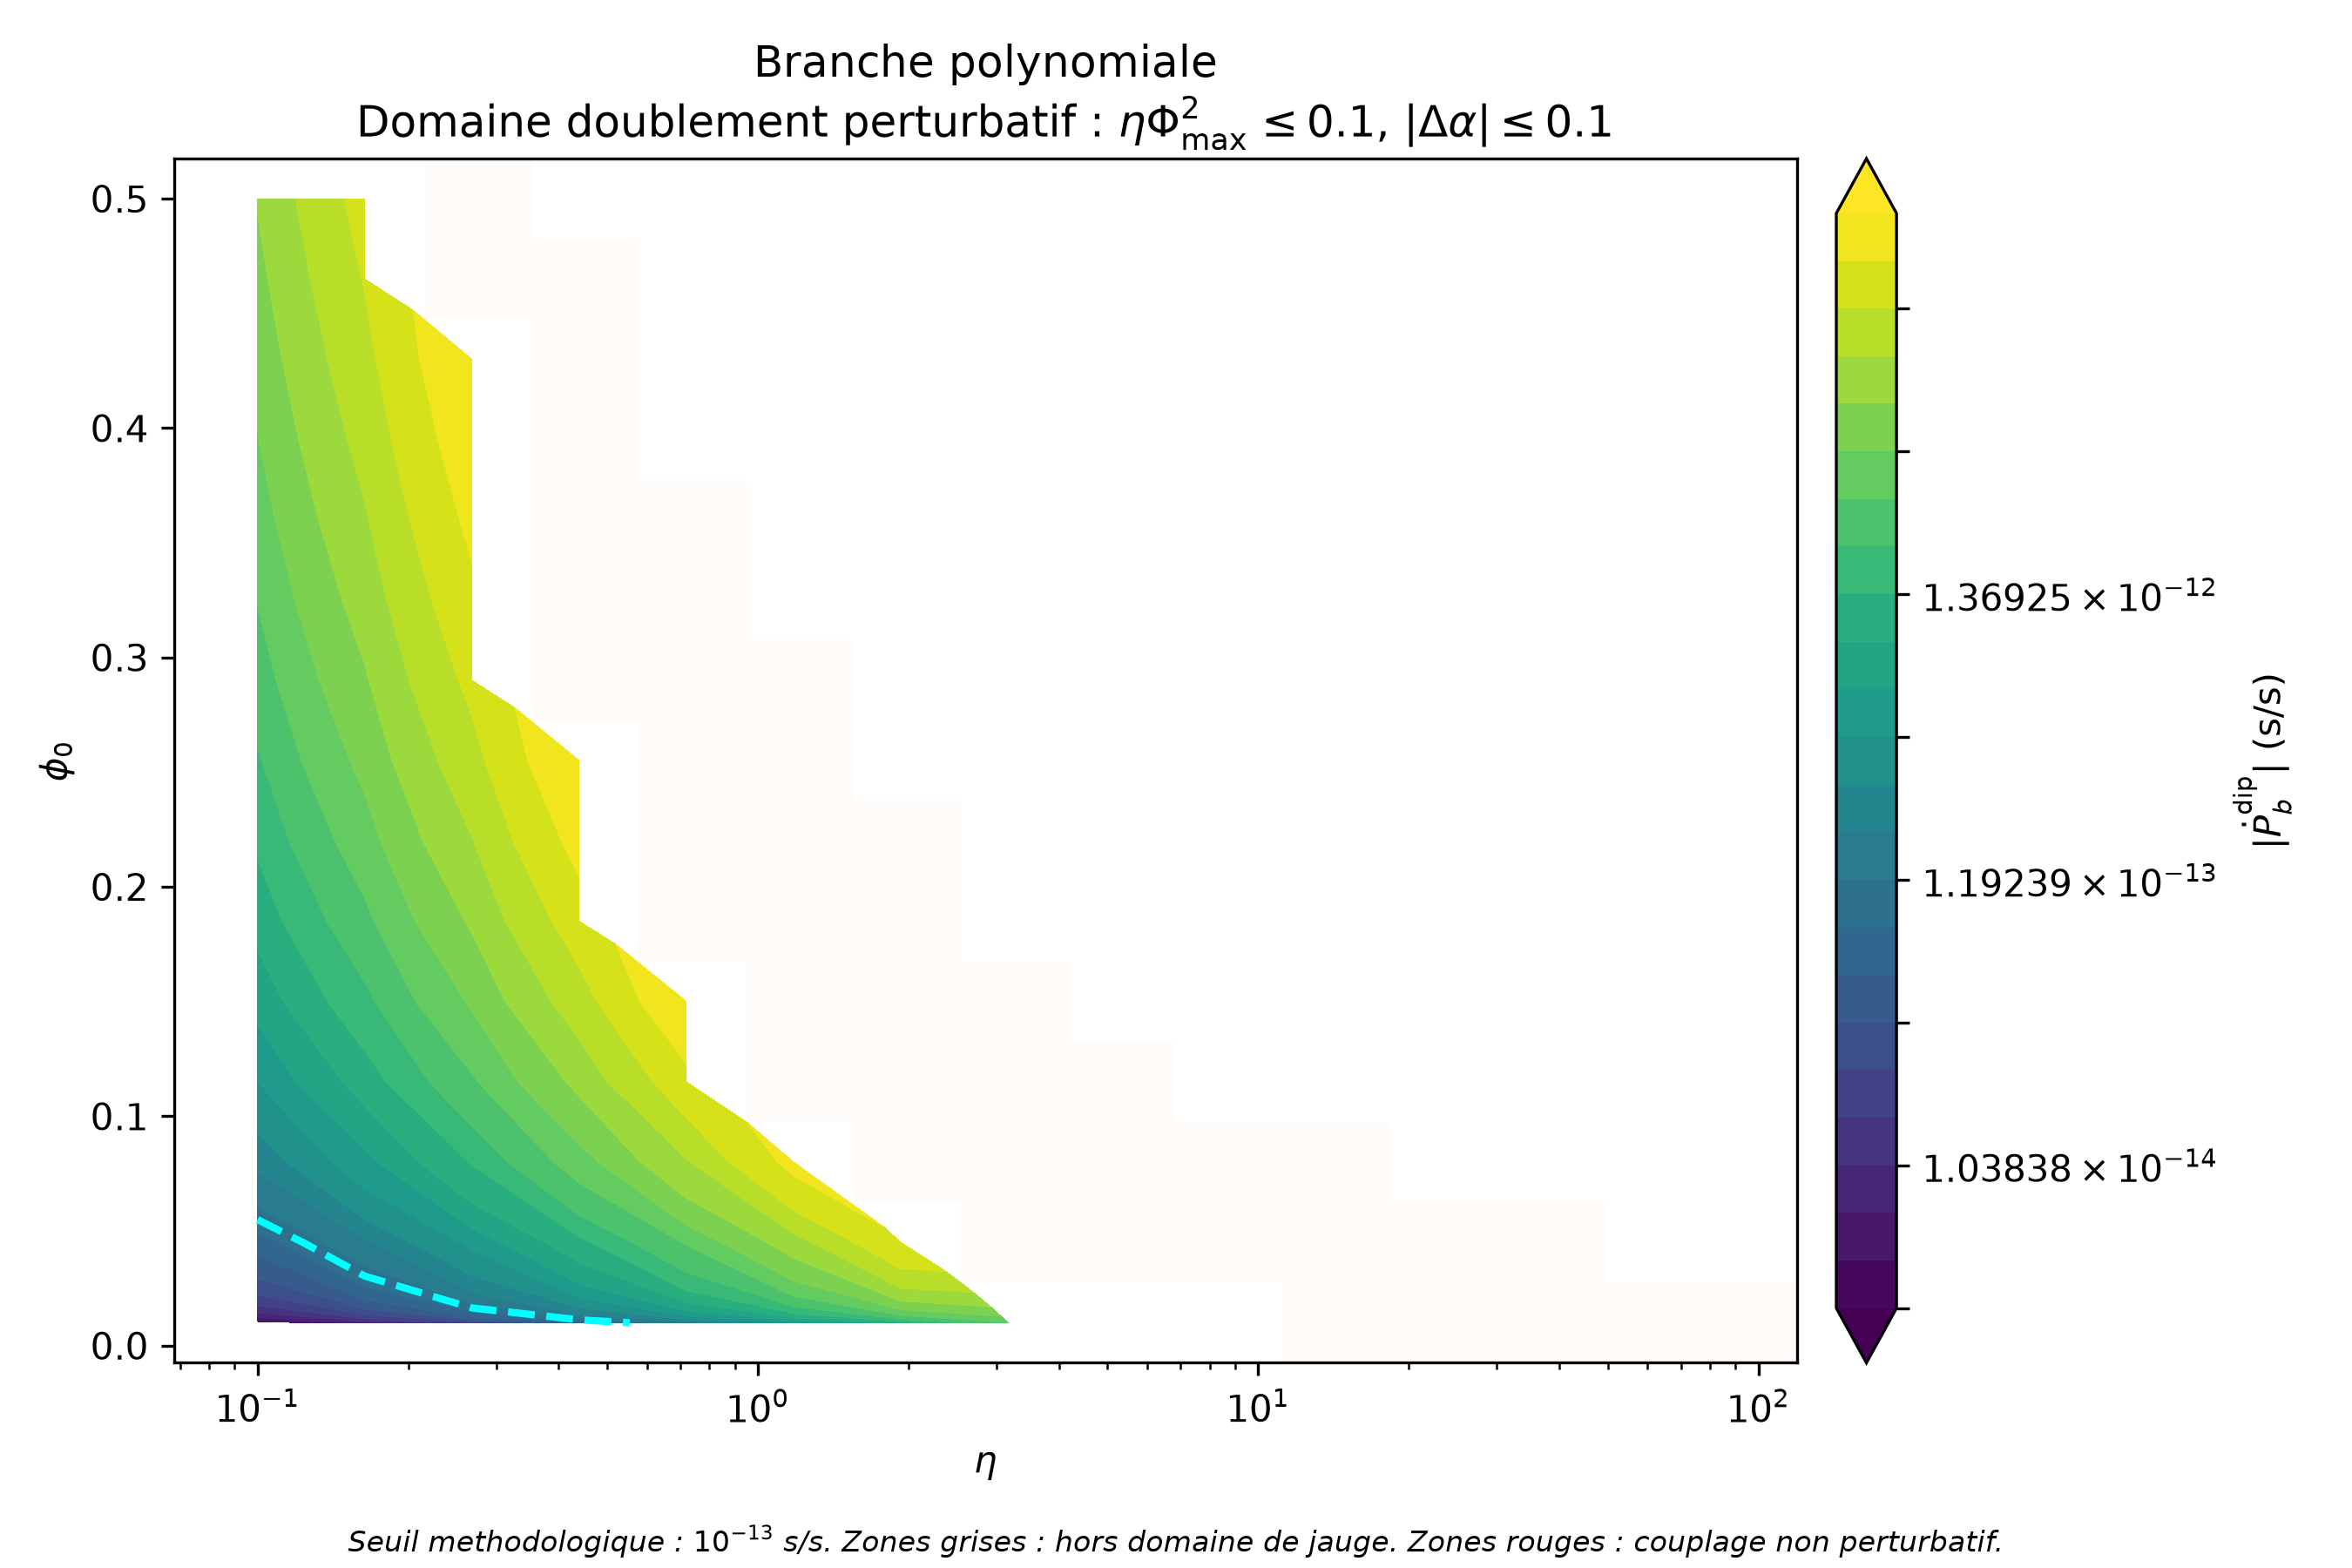
\includegraphics[width=0.48\textwidth]{figures/pulsar_field_sensitivity_heatmap_polynomial.png}
  \caption{Cartes de sensibilité numérique du pipeline SCCI-2026. À gauche : balayage standard. À droite : paramétrisation polynomiale $\mathfrak R(\Phi)=1+\eta\Phi^2$, avec exclusion des configurations hors domaine perturbatif ou à couplage différentiel non perturbatif.}
  \label{fig:heatmaps_scci_2026}
\end{figure}

\section{Action effective et équation du champ}

Considérons l'action effective :

\begin{equation}
S_{\mathrm{eff}}
=
\int \mathrm d^4x\sqrt{-g}
\left[
\frac{M_{\mathrm{Pl}}^2}{2}f(R,\Phi)
-\frac12K^{ab}(\Phi)\nabla_a\Phi\nabla_b\Phi
-V(\Phi)
-\frac14Z_A(\Phi)\operatorname{Tr}(F_{\mu\nu}F^{\mu\nu})
\right]
+S_{\mathrm{mat}} .
\end{equation}

La variation par rapport à $\Phi$ donne :

\begin{equation}
\nabla_a\left[K^{ab}(\Phi)\nabla_b\Phi\right]
-\frac12\frac{\partial K^{cd}}{\partial\Phi}\nabla_c\Phi\nabla_d\Phi
-\frac{\partial V}{\partial\Phi}
+\frac{M_{\mathrm{Pl}}^2}{2}\frac{\partial f}{\partial\Phi}
-\frac14\frac{\partial Z_A}{\partial\Phi}
\operatorname{Tr}(F_{\mu\nu}F^{\mu\nu})
+\mathcal S_{\mathrm{mat}}
=0 .
\end{equation}

La paramétrisation polynomiale

\begin{equation}
\mathfrak R(\Phi)=1+\eta\Phi^2
\end{equation}

est cohérente avec un couplage minimal de jauge à une boucle sous l'hypothèse d'identification $\mathfrak R\equiv Z_A$. Son statut de dérivation reste conditionné à cette hypothèse et à la validité du développement perturbatif.

\section{Contribution dipolaire et garde-fous}

Une asymétrie de couplage

\begin{equation}
\Delta\alpha=\alpha_B-\alpha_A\neq0
\end{equation}

entraîne une contribution dipolaire de la forme générale :

\begin{equation}
\dot P_b^{\mathrm{dip}}
=
-\mathcal G_{\mathrm{dip}}
(\Delta\alpha)^2
\mathcal K_{\mathrm{orb}} .
\end{equation}

Pour la paramétrisation polynomiale, les bornes perturbatives sont :

\begin{equation}
\eta\Phi_{\max}^2\le0{,}1
\qquad\text{et}\qquad
|\Delta\alpha|\le0{,}1 .
\end{equation}

Tout dépassement de ces bornes traduit une perte de validité de l'approximation, et non une prédiction physique.

Le repère de \SI{1e-13}{\second\per\second} constitue un critère interne de sensibilité numérique du pipeline, et non une contrainte observationnelle établie.

\section{Perspective ab initio}

Le passage d'une analyse de sensibilité paramétrique à une prédiction ab initio exige de dériver $\mathfrak R$, $\sigma_i$, $\mathcal N_\Phi$ et $\mathcal G_{\mathrm{dip}}$ à partir de la variation de l'action complète SCCI-2026.

Tant que cette dérivation n'est pas réalisée, les valeurs de $\alpha_i$ et de $\dot P_b^{\mathrm{dip}}$ restent des quantités de sensibilité, et non des prédictions observationnelles.

\end{document}
